\todo[inline, color=pink, size=normalsize]{Descrição geral do problema}

O problema do estacionamento paralelo consiste na determinação da trajetória a ser percorrida por um veículo durante a realização de uma manobra de baliza, a partir do qual objetiva-se o posicionamento do automóvel em uma vaga paralela à via \cite{paromtchik_autonomous_1996}. Neste procedimento, é necessário que sejam impostas limitações à velocidade e à aceleração do automóvel de forma a garantir o conforto dos passageiros e evitar o choque com outros veículos já estacionados ou com os limites delimitados na via \cite{li_time-optimal_2016}. Assim, pretende-se determinar a trajetória a ser percorrida por um veículo para que a referida manobra seja realizada no menor tempo possível \cite{li_time-optimal_2016}. As variáveis empregadas na formulação do problema, bem como as posições inicial e final do automóvel são representadas nas Figuras \ref{fig:estacionamento:estacionamento} e \ref{fig:estacionamento:estacionamentoVia}, respectivamente.

\noindent	
\begin{minipage}{\textwidth}
	\vspace{\onelineskip}
	\centering
	\includegraphics[scale=0.14]{draw/resultados/pdf/estacionamento}
	\captionof{figure}[Representação esquemática das variáveis empregadas na formulação do problema do estacionamento]{Representação esquemática das variáveis empregadas na formulação do estudo de caso em análise.}
	\label{fig:estacionamento:estacionamento}
	\vspace{\onelineskip}
\end{minipage}

\noindent	
\begin{minipage}{\textwidth}
	\vspace{\onelineskip}
	\centering
	\includegraphics[scale=0.14]{draw/resultados/pdf/estacionamentoVia}
	\captionof{figure}[Posições inicial e final do automóvel e  dimensões da via e da vaga]{Posições inicial e final do automóvel e dimensões da via e da vaga.}
	\label{fig:estacionamento:estacionamentoVia}
	\vspace{\onelineskip}
\end{minipage}

Nestas figuras tem-se que $ l $ é a distância entre os eixos do veículo, $ m $ e $ n $ são os afastamentos entre as extremidades do automóvel e os eixos traseiro e dianteiro, respectivamente, enquanto  que $ b $ é metade da largura do mesmo. A velocidade e aceleração do ponto médio $ P(d_x, d_y) $ referente ao eixo traseiro são representadas por $ v(t) $ e $ a(t) $, respectivamente. Os pontos $ A(t) $, $ B(t) $, $ C(t) $ e $ D(t) $ são as extremidades do retângulo que delimita o veículo. O ângulo entre a velocidade do ponto médio do eixo dianteiro e a reta $ \gamma $ é dado por $ \phi(t) $. A inclinação de $ \gamma $ em relação ao eixo $ x $ é dada por $ \theta(t) $. O \textit{jerk} (ou sobre-aceleração) e a velocidade angular referente à $\phi(t)$ são denotados respectivamente por $ j(t) $ e $ \omega(t) $. A vaga na qual o veículo deve estacionar possui comprimento $ SL $ e largura $ SW $, enquanto a via na qual se encontra possui largura $ CL $. O centro instantâneo de rotação é representado pelo ponto $ CIR $. 

\todo[inline, color=pink, size=normalsize]{Descrição geral do problema - Comparação com os resultados originais}

As trajetórias de controle reportadas por \citeonline{li_time-optimal_2016} são apresentadas na Figura \ref{fig:estacionamento:original}. Tais trajetórias apresentam oscilações de alta frequência sempre que verificam-se variações bruscas em $ j(t) $ ou em $ \omega(t) $. Logo, espera-se que tais oscilações apareçam nos resultados associados aos métodos aqui avaliados, o que representa um desafio para qualquer \textit{solver} de controle ótimo. 

\noindent	
\begin{minipage}{\textwidth}
	\vspace{\onelineskip}
	\centering
	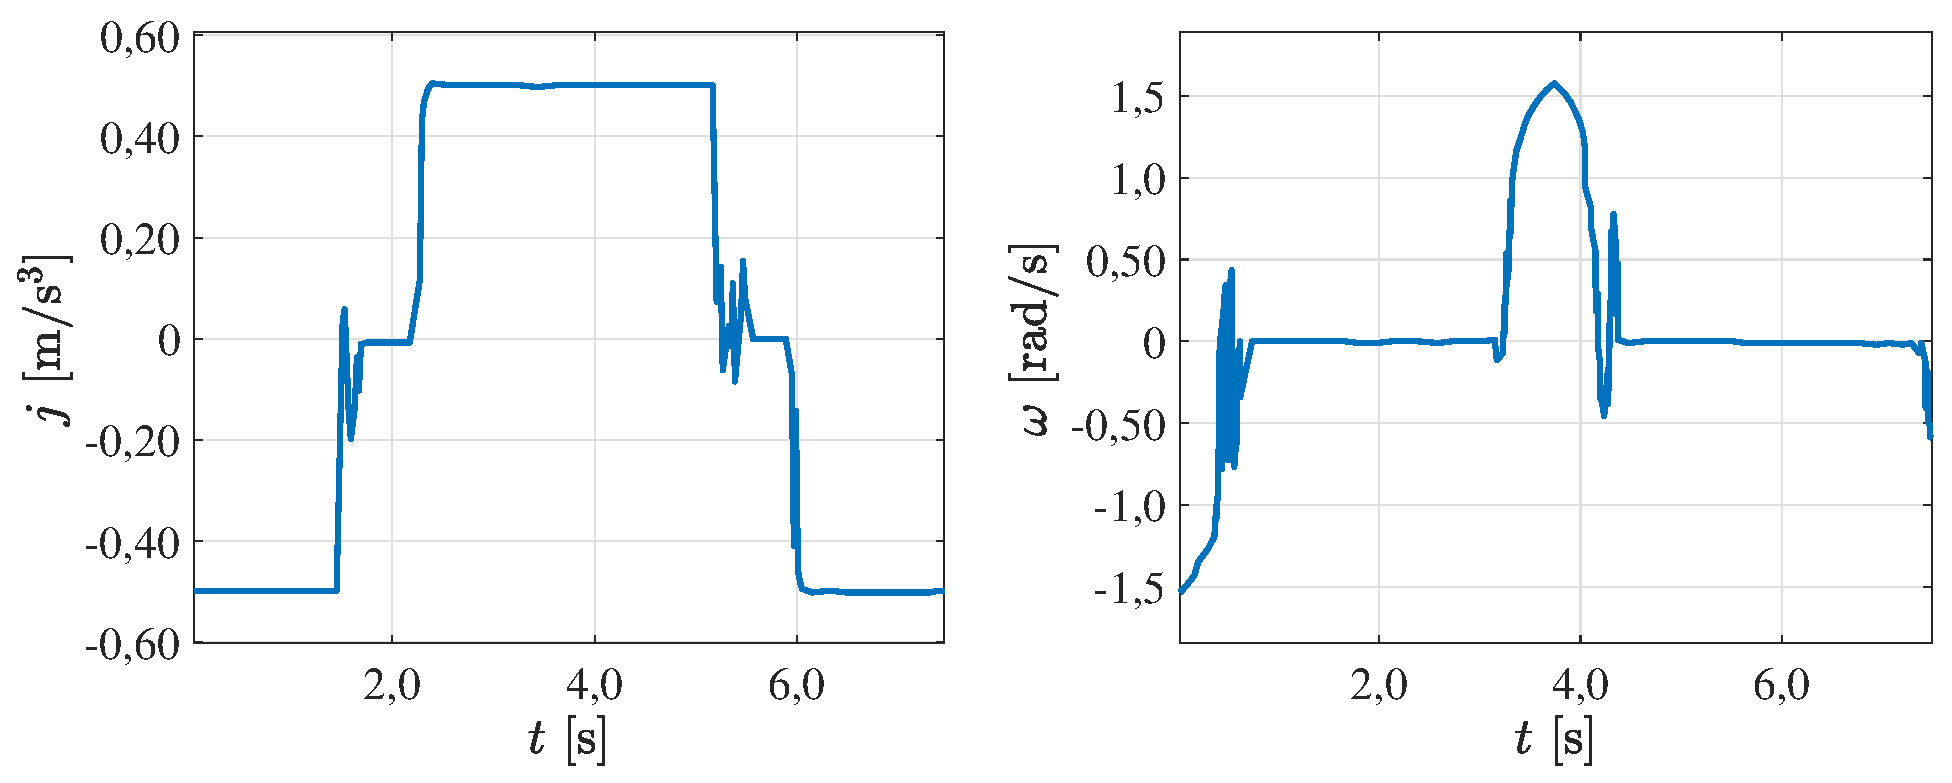
\includegraphics[scale=0.42]{fig/resultados/estacionamento/obs/original}
	\captionof{figure}[Trajetórias de controle para o problema do estacionamento reportadas pela literatura]{Trajetórias de controle para o problema do estacionamento reportadas por \citeonline{li_time-optimal_2016}.}
	\label{fig:estacionamento:original}
	\vspace{\onelineskip}
\end{minipage}

\todo[inline, color=pink, size=normalsize]{Apresentação da função objetivo}

A função objetivo a ser minimizada nesta aplicação é dada como \cite{li_time-optimal_2016}:
%
\begin{equation}
	\label{eq:estacionamento:J}
	J = t_f
\end{equation}
%
sujeito ao seguinte conjunto de restrições:
%
\begin{subequations}
\begin{equation}
\label{eq:estacionamento:dinamica}
\dot{d}_x(t) = v(t) \cos(\theta(t)),\;\;d_x(0) = SL\;\text{m}
\end{equation}
\vspace{-0.6cm}
\begin{equation}
\dot{d}_y(t) = v(t)\sin(\theta(t)),\;\; d_y(0) = d_{y0} \; \text{m}
\end{equation}
\vspace{-0.5cm}
\begin{equation}
\dot{v}(t) = a(t),\;\; v(0) = 0 \; \text{m/s}
\end{equation}
\vspace{-0.55cm}
\begin{equation}
\dot{a}(t) = j(t),\;\;  a(0) = 0 \; \text{m/s$^2$}
\end{equation}
\vspace{-0.3cm}
\begin{equation}
\dot{\theta}(t) = \frac{v(t) \tan(\phi(t))}{l},\;\;  \theta(0) = 0 \; \text{rad}
\end{equation}
\vspace{-0.5cm}
\begin{equation}
\dot{\phi}(t) = \omega(t),\;\;  \phi(0) = 0 \; \text{rad} 
\end{equation}
\end{subequations}
%
em que $t$ é o tempo ($ t_f $ é o tempo final), $ \mathbf{x}(t) = \begin{bmatrix} d_x(t) & d_y(t) & v(t) & a(t) & \theta(t) & \phi(t) \end{bmatrix}^T $ é o vetor de variáveis de estados e $ \mathbf{u}(t) = \begin{bmatrix} j(t) & \omega(t) \end{bmatrix}^T $ é o vetor de variáveis de controle.

\todo[inline, color=pink, size=normalsize]{Apresentação das restrições - Restrições laterais}

Visando garantir o conforto dos passageiros e reduzir o estresse sobre os atuadores, são impostas as restrições:
%
\begin{subequations}
\begin{equation}
\label{eq:estacionamento:laterais}
|a(t)| \leq 0,75 \text{ m/s$^2$} 
\end{equation}
\vspace{-0.6cm}
\begin{equation}
|v(t)| \leq 2 \text{ m/s} 
\end{equation}
\vspace{-0.6cm}
\begin{equation}
|\phi(t)| \leq 0,58 \text{ rad} 
\end{equation}
\vspace{-0.6cm}
\begin{equation}
|\kappa'(t)| \leq 0,6 \text{ 1/(m $\cdot$ s)} 
\end{equation}
\vspace{-0.6cm}
\begin{equation}
|j(t)| \leq  0,5 \text{ m/s$^3$}
\end{equation}
\end{subequations}
%
\noindent em que $ \kappa'(t) = \omega(t)/(l \cos^2(\phi(t))) $ é a derivada referente à curvatura instantânea. Observa-se que, restringindo-se $ \kappa'(t) $ restringe-se automaticamente $ \omega(t) $.

\todo[inline, color=pink, size=normalsize]{Apresentação das restrições - Restrições terminais}

Assume-se que ao fim da execução da manobra o veículo deve estar parado, paralelo à via e posicionado no interior da vaga. Para tanto, devem ser satisfeitas as restrições terminais:
%
\begin{subequations}
\begin{equation}
\label{eq:estacionamento:terminais}
m \leq d_x(t_f) \leq SL - (l + n)
\end{equation}
\vspace{-0.7cm}
\begin{equation}
- (SW - b) \leq d_y(t_f) \leq -b
\end{equation}
\vspace{-0.65cm}
\begin{equation}
v(t_f) = 0 \; \text{m/s} 
\end{equation}
\vspace{-0.7cm}
\begin{equation}
a(t_f) = 0 \; \text{m/s$^2$}
\end{equation}
\vspace{-0.7cm}
\begin{equation}
\theta(t_f) = 0 \; \text{rad}
\end{equation}
\end{subequations}

\todo[inline, color=pink, size=normalsize]{Apresentação das restrições - Restrições de caminho}

Todas as posições do veículo durante a execução da manobra devem estar contidas na região delimitada pelas curvas $ \alpha(x) = (U_s(x - SL) - U_s(x)) \, SW $ e $ \beta(x) = CL $, sendo $ U_s(x) $ a função degrau unitário. Dadas as relações entre a posição do veículo e os pontos $ A $, $ B $, $ C $ e $ D $,
%
\begin{subequations}
\begin{equation}
\label{eq:estacionamento:abcd}
A = (A_x, A_y) = (d_x + (l+n) \cos(\theta) - b \sin(\theta), \; d_y + (l+n) \sin(\theta) + b \cos(\theta)) 
\end{equation}
\vspace{-1.1cm}
\begin{equation}
B = (B_x, B_y) = (d_x + (l+n) \cos(\theta) + b \sin(\theta), \; d_y + (l+n) \sin(\theta) - b \cos(\theta))
\end{equation}
\vspace{-0.75cm}
\begin{equation}
C = (C_x, C_y) = (d_x - m \cos(\theta) + b \sin(\theta), \; d_y - m \sin(\theta) - b \cos(\theta))
\end{equation}
\vspace{-0.65cm}
\begin{equation}
D = (D_x, D_y) = (d_x - m \cos(\theta) - b \sin(\theta), \; d_y - m \sin(\theta) + b \cos(\theta))
\end{equation}
\end{subequations}
%
é possível formular as seguintes restrições para garantir que o veículo não se choque com os limites da via ou da vaga:
%
\begin{subequations}
\begin{equation}
	\label{eq:estacionamento:choqueViaVaga}
A_y(t) \leq \beta(A_x)
\end{equation}
\vspace{-0.7cm}
\begin{equation}
B_y(t) \leq \beta(B_x)
\end{equation}
\vspace{-0.7cm}
\begin{equation}
C_y(t) \leq \beta(C_x)
\end{equation}
\vspace{-0.7cm}
\begin{equation}
D_y(t) \leq \beta(D_x)
\end{equation}
\vspace{-0.7cm}
\begin{equation}
A_y(t) \geq \alpha(A_x)
\end{equation}
\vspace{-0.7cm}
\begin{equation}
B_y(t) \geq \alpha(B_x)
\end{equation}
\vspace{-0.7cm}
\begin{equation}
C_y(t) \geq \alpha(C_x)
\end{equation}
\vspace{-0.7cm}
\begin{equation}
D_y(t) \geq \alpha(D_x) 
\end{equation}
\end{subequations}

Como indicado na Figura \ref{fig:estacionamento:choqueVia} é possível que exitam colisões mesmo que as restrições apresentadas sejam respeitadas.

\noindent	
\begin{minipage}{\textwidth}
	\vspace{\onelineskip}
	\centering
	\includegraphics[scale=0.16]{draw/resultados/pdf/estacionamentoQuina}
	\captionof{figure}[Situação em que o veículo se choca com os limites da vaga]{Situação em que as restrições são satisfeitas e o veículo ainda assim se choca com os limites da vaga.}
	\label{fig:estacionamento:choqueVia}
	\vspace{\onelineskip}
\end{minipage}

Neste caso, considerando um novo sistema de coordenadas $ x'Gy' $ partindo do centro do veículo, redefinem-se os pontos $ O $ e $ E $ da seguinte forma:
%
\begin{subequations}
\begin{equation}
O_{x'Gy'} = (O_x', O_y') = (-d_x \cos(\theta) - d_y \sin(\theta) - \frac{l + n - m}{2}, \; d_x \sin(\theta) - d_y \cos(\theta)) 
\end{equation}
\vspace{-0.55cm}
\begin{equation}
E_{x'Gy'} = (E_x', E_y') = (-d_x \cos(\theta) - d_y \sin(\theta) - \frac{l + n - m}{2} + SL \cos(\theta),\nonumber 
\end{equation}
\vspace{-0.7cm}
\begin{equation}
d_x \sin(\theta) - d_y \cos(\theta) - SL \sin(\theta))
\end{equation}
\end{subequations}

Logo, para garantir que as laterais do automóvel não se choquem com os pontos $ O $ e $ E $ durante a execução da manobra, deve-se admitir que: 
%
\begin{subequations}
\begin{equation}
\label{eq:estacionamento:choqueQuinaVaga}
|O_x'| \geq \frac{l + m + n}{2} \;\; \text{quando } |O_y'| \leq b 
\end{equation}
\vspace{-0.7cm}
\begin{equation}
\label{eq:estacionamento:choqueQuinaVagab}
|E_x'| \geq \frac{l + m + n}{2} \;\; \text{quando } |E_y'| \leq b 
\end{equation}
\end{subequations}

\todo[inline, color=pink, size=normalsize]{Tabela das constantes do problema}

A seguir estão listados os parâmetros utilizados para a resolução deste estudo de caso \cite{li_time-optimal_2016}: posição inicial do ponto médio do eixo traseiro na direção $y$ ($ d_{y0} = 1,5 $), distância entre os eixos do veículo ($ l = 2,588$ m), distância entre o eixo dianteiro e a dianteira do veículo ($ n = 0,839 $ m), distância entre o eixo traseiro e a traseira do veículo ($ m = 0,657 $ m), metade da largura do automóvel ($ b = 0,8855 $ m), comprimento da vaga ($ SL = 6 $ m), largura da vaga ($ SW = 2 $ m) e largura da via ($ CL = 3,5 $ m).

\todo[inline, color=pink, size=normalsize]{Considerações específicas de cada problema - Aproximações para as funções descontínuas}

Conforme destacado por \citeonline{li_time-optimal_2016}, a resolução do estudo de caso em análise pode ainda ser dificultada pela representação matemática dos limites da vaga, que possui descontinuidades em $ x = 0 $ e $ x = SL $. Para evitar a divergência do processo de otimização, os limites da vaga são aqui representados pela soma de funções sigmoides, conforme a Figura \ref{fig:estacionamento:aproximacaoVaga}. 

\noindent	
\begin{minipage}{\textwidth}
	\vspace{\onelineskip}
	\centering
	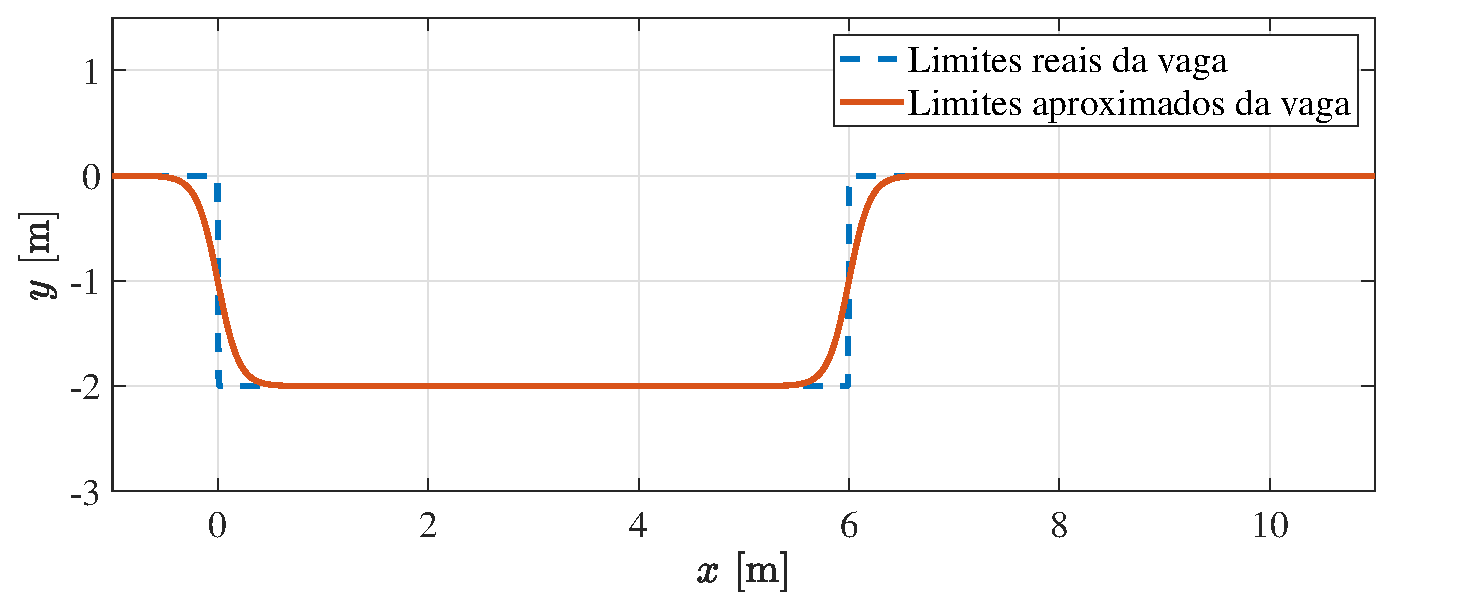
\includegraphics[scale=0.58]{fig/resultados/estacionamento/obs/vaga}
	\captionof{figure}[Representação geométrica adotada para a  representação dos limites da vaga]{Representação geométrica adotada para a  representação dos limites da vaga.}
	\label{fig:estacionamento:aproximacaoVaga}
	\vspace{\onelineskip}
\end{minipage}

Neste caso, considera-se:
%
\begin{equation}
\alpha(x) = \big(-sigm(x, 0) + sigm(x, SL)\big) \, SW
\end{equation} 
%
em que $ sigm(x, c) $ é a função sigmoide, dada como:
%
\begin{equation}
	sigm(x, c) = \frac{1}{1 + e^{-10 \, (x - c)}}
\end{equation} 
%
em que o parâmetro $ -10 $, que multiplica o expoente no denominador, foi escolhido ivia experimentação numérica. 

De forma análoga, destacam-se descontinuidades associadas às Equações \eqref{eq:estacionamento:choqueQuinaVaga} e \eqref{eq:estacionamento:choqueQuinaVagab}, uma vez que a definição das mesmas depende da função módulo e de uma condição de ativação, sendo a primeira válida apenas para $ |O_y'| \leq b $ e a segunda somente quando $ |E_y'| \leq b $. 

Para tratar as descontinuidades atribuídas à presença da função módulo, basta que a mesma seja reescrita da seguinte forma:
%
\begin{equation}
	|z| \equiv z \, g(z)
\end{equation}
%
sendo:
%
\begin{equation}
	g(z) = \begin{cases} 1, & \mbox{se } z \geq 0 \\ -1, & \mbox{se } z < 0 \end{cases}
\end{equation}

Deve-se então aproximar $ g(z) $ por meio da função tangente hiperbólica $\tanh(z) $, conforme ilustrado na Figura \ref{fig:estacionamento:aproximacaoModulo}.
\begin{equation}
	\label{eq:estacionamento:aproximacaoModulo}
	|z| \approx z \tanh(z)
\end{equation}
%
em que:
%
\begin{equation}
	\tanh(z) = \frac{e^{10z} - 1}{e^{10z} + 1}
\end{equation}
%
onde o parâmetro $ -10 $, que multiplica os expoentes do numerador e denominador, foi escolhido via experimentação numérica. 

\noindent	
\begin{minipage}{\textwidth}
	\vspace{\onelineskip}
	\centering
	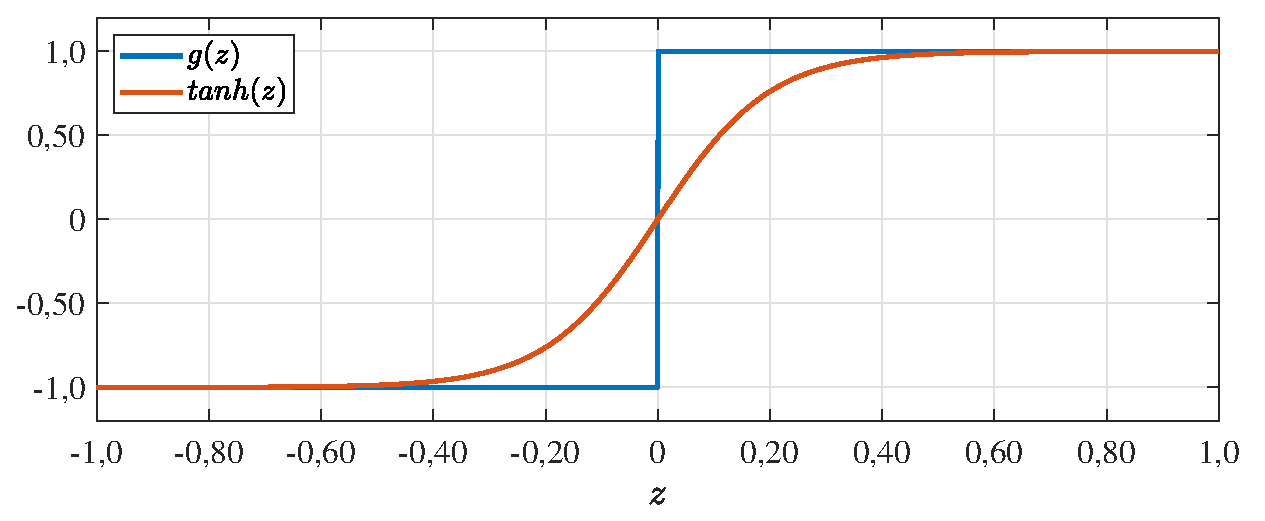
\includegraphics[scale=0.58]{fig/resultados/estacionamento/obs/apxMod}
	\captionof{figure}[Representação geométrica das funções usadas para a aproximação da função módulo]{Representação geométrica das funções $ g(z) $ e $ \tanh(z) $ usadas para a aproximação da função módulo.}
	\label{fig:estacionamento:aproximacaoModulo}
	\vspace{\onelineskip}
\end{minipage}

Resta agora tratar as descontinuidades atribuídas às condições de ativação associadas às Equações \eqref{eq:estacionamento:choqueQuinaVaga} e \eqref{eq:estacionamento:choqueQuinaVagab}. Para essa finalidade, considerando a princípio a primeira restrição, a mesma deve ser reescrita levando-se em conta a aproximação apresentada na Equação \eqref{eq:estacionamento:aproximacaoModulo}:
%
\begin{gather}
|O_x'| \geq \frac{l + m + n}{2}, \;\; \text{quando } |O_y'| \leq b \\ 
O_x' \tanh(O_x') \geq \frac{l + m + n}{2}, \;\; \text{quando } -b \leq O_y' \leq b
\end{gather}

Propõe-se então que a condição de ativação associada à restrição em questão seja representada por uma função $ h(z) $ da forma que:
%
\begin{equation}
	h(z) = \begin{cases} \infty, & \mbox{se } z < -b \\ 1, & \mbox{se } -b \leq z \leq b \\  \infty, & \mbox{se } z > -b \end{cases}
\end{equation}
% 
onde:
\begin{gather}
\label{eq:estacionamento:restricaoBandPass}
O_x' \tanh(O_x') \geq \frac{l + m + n}{2}, \;\; \text{quando } -b \leq O_y' \leq b \\
\label{eq:estacionamento:restricaoBandPassb}
O_x' \tanh(O_x') \, h(O_y) \geq \frac{l + m + n}{2}
\end{gather}

Observe que caso $ O_y' < -b$ ou $O_y' > b $, a Equação  \eqref{eq:estacionamento:restricaoBandPassb} se reduz a $ \infty \geq \frac{l + m + n}{2} $, que claramente é satisfeita para qualquer $ O_x' $. Caso contrário, tal restrição se reduz a $ O_x' \tanh(O_x') \geq (l + m + n)/2 $. Logo, conclui-se que as Equações \eqref{eq:estacionamento:choqueQuinaVaga} e \eqref{eq:estacionamento:restricaoBandPassb} são equivalentes. 

Basta agora que a função $ h(z) $ seja aproximada por um somatório de sigmoides, conforme ilustrado na Figura \ref{fig:estacionamento:bandPass}:

\noindent	
\begin{minipage}{\textwidth}
	\vspace{\onelineskip}
	\centering
	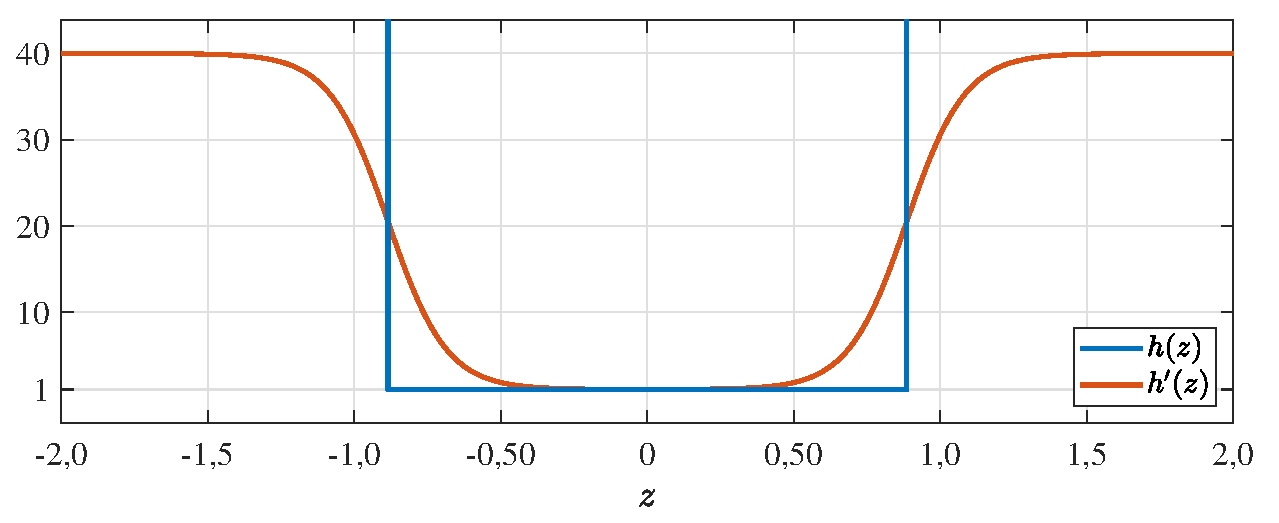
\includegraphics[scale=0.58]{fig/resultados/estacionamento/obs/apxBandPass}
	\captionof{figure}[Representação geométrica das funções $ h(z) $ e $ h'(z) $ usadas para evitar o choque entre o veículo e a vaga]{Representação geométrica das funções usadas para evitar o choque entre o veículo e a vaga.}
	\label{fig:estacionamento:bandPass}
	\vspace{\onelineskip}
\end{minipage}

Neste caso tem-se \cite{li_time-optimal_2016}:
%
\begin{equation}
	h(z) \approx h'(z) = 1 + 39 \big(1 + sigm(x, b) - sigm(x, -b)\big)
\end{equation}

Vale ressaltar que, uma vez que não é possível fazer $ h(z) = \infty $ para $ z < -b $ ou $ z > b $, adotou-se, após um processo de experimentação numérica, $ h'(z) = 40 $ nesse intervalo. 

Analogamente para a restrição associada à $ E'_x $: 
%
\begin{gather}
|E_x'| \geq \frac{l + m + n}{2} \;\; \text{quando } |E_y'| \leq b  \\
E_x' \tanh(E_x') \, h(E_y) \geq \frac{l + m + n}{2}
\end{gather}

\todo[inline, color=pink, size=normalsize]{Considerações específicas de cada problema - Inicialização do problema com duas execuções}

Para a obtenção de uma trajetória factível, \citeonline{li_time-optimal_2016} propuseram a inclusão de uma região crítica, delimitada pelos pontos $ X $, $ Y $, $ Z $ e $ W $, conforme apresentado na Figura \ref{fig:estacionamento:estacionamentoVia}, e a resolução de uma série de $ N_{fe} $ PCOs semelhantes ao original. Na formulação do $ N_\chi $-ésimo PCO consideram-se restrições que garantem que veículo esteja contida na região crítica para $ t \in [h \, N_\chi, \; tf] $, sendo $ h = t_f/N_{fe} $ e $ N_\chi = 1, ..., N_{fe} $. Então, a solução do primeiro PCO é utilizada como estimativa inicial para resolução do segundo, e assim sucessivamente, até que o PCO original seja resolvido para $ N_\chi = N_{fe} $. 

Visando minimizar o esforço computacional envolvido na inicialização do PPNL, uma abordagem distinta foi aqui proposta. Cada uma das soluções aqui apresentadas foram obtidas a partir de duas execuções. Na primeira, desconsideram-se todas as restrições, uma vez que estas não são convexas e dificultam a obtenção de trajetórias viáveis. Então, na segunda execução, as restrições inicialmente desconsideradas são inseridas no problema e a solução obtida anteriormente é utilizada na inicialização do vetor de variáveis de estado e de controle. O tempo de processamento $ t_p $ e o número de avaliações da função objetivo $ n_{aval} $ atribuídos a cada solução foram computados a partir da soma destas duas etapas. Vale ressaltar que, para que uma solução seja determinada, ambas as execuções devem ser bem sucedidas.

\todo[inline, color=pink, size=normalsize]{Apresentação da análise de sensibilidade $ J \times N $ para definição de $ N_m $ }

São apresentados na Figura \ref{fig:estacionamento:sensibilidade:J} os resultados obtidos considerando a influência de $N$ no valor da função objetivo (melhor solução encontrada para cada valor de $N$), bem como o número mínimo de nós de colocação $ N_m $. Neste caso também foram utilizados trinta valores distintos para $N$, linearmente espaçados entre 5 e 150. \textcolor{red}{O valor da função objetivo reportado por XXXXX para este problema é .... unidade.}

\noindent	
\begin{minipage}{\textwidth}
	\vspace{\onelineskip}
	\centering
	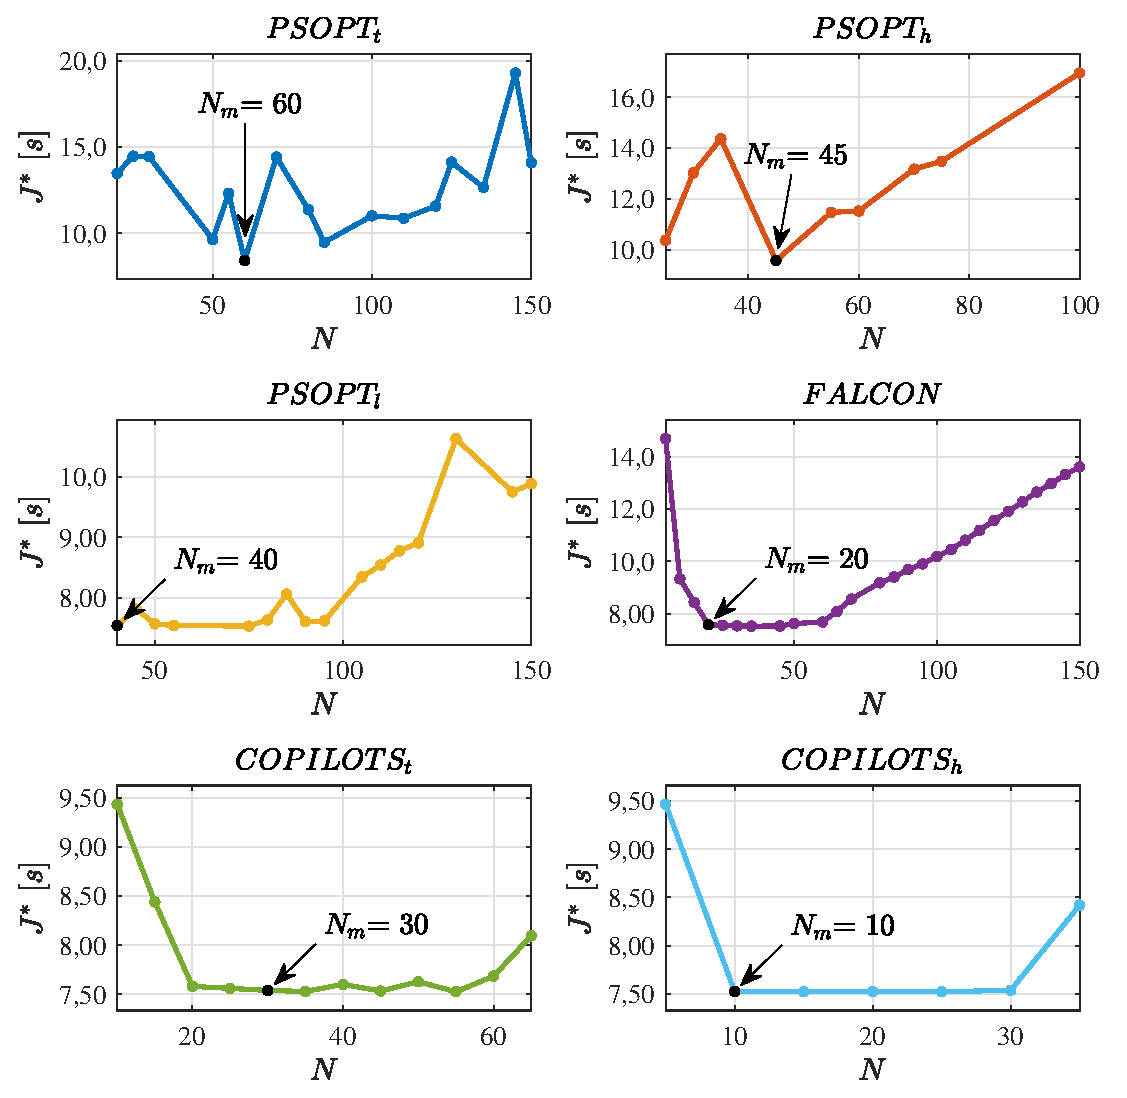
\includegraphics[scale=0.7]{fig/resultados/estacionamento/sens/J}
	\captionof{figure}[Influência do número de nós de colocação $ N $ valor da função objetivo $ J^* $ para o problemas do estacionamento]{Influência do número de nós de colocação valor da função objetivo para o problemas do estacionamento.}
	\label{fig:estacionamento:sensibilidade:J}
	\vspace{\onelineskip}
\end{minipage}

\todo[inline, color=pink, size=normalsize]{Análise da análise de sensibilidade $ J \times N $}

Nesta figura percebe-se a dificuldade inerente existente neste estudo de caso, isto é; todos os pacotes considerados não conseguem, para todos os valores de $N$ utilizados, obter a solução deste problema. À  medida que o valor de $N$ aumenta, verifica-se que o valor de $J^*$ diminui a princípio para, em seguida, voltar a aumentar. Verifica-se que esse comportamento nos resultados associados a todos os métodos, com exceção do $PSOPT_l$.  Uma vez que aumenta-se $N$, a inicialização dos pacotes se torna mais crítica, dificultando a inicialização do PCO. O crescimento simultâneo de $J^*$ e $N$ indica que o estudo de caso em análise é consideravelmente sensível as estimativas iniciais, provavelmente por conta do alto número de restrições associadas ao mesmo. Uma vez que $J^*$ não converge com o aumento de $N$, atribuiu-se a $N_m$ o $N$ ao qual estiver associado o menor $J^*$.

Cabe ressaltar que não foi possível resolver o problema via $PSOPT_l$ para $N < 40$. No caso desse tipo de colocação, quando maior o $N$, maior será o polinômio empregado na representação dos estados e controles. A complexidade das trajetórias envolvidas, assim como o alto número de estados e controles, provavelmente, impossibilita que o mesmo seja resolvido por meio do emprego de polinômios de baixa ordem.

Somente empregando o $FALCON$, o $COPILOTS_h$ e o $COPILOTS_t$ foi possível resolver o problema para menores valores de $N$, sendo os menores valores iguais a 5, 5 e 10, respectivamente. Em contrapartida,  os valores mínimos para $N$ associados ao $PSOPT_t$ e ao $PSOPT_h$ são iguais a 20 e 25, respectivamente, sendo maiores que aqueles requeridos pelo $FALCON$ e pelo $COPILOTS$. Tal diferença pode ser justificada pela dificuldade encontrada pelo otimizador empregado pelo $PSOPT$ (Método de Ponto Interior).

O máximo valor de $N$ associado ao $PSOPT_h$ (100) é maior que aquele requerido pelo $PSOPT_t$ (150). O mesmo pode ser observado no que tange os máximos valores de $N$ associados ao $COPILOTS_t$ (65) e ao $COPILOTS_h$ (35). As diferenças entre os valores máximos de $N$ para os métodos que usam as colocações trapezoidal e de Hermite-Simpson, se deve às propriedades numéricas inerentes a cada tipo de colocação. Vale ressaltar que a implementação da colocação Hermite-Simpson depende da determinação de pontos médios entre os nós de colocação, o que aumenta o número de variáveis a serem inicializadas e determinadas no processo de otimização. Cabe ressaltar que os máximos valores de $N$ requeridos pelo $COPILOTS_t$ e pelo $COPILOTS_h$ são bem menores que aqueles associados aos demais métodos. 

\todo[inline, color=pink, size=normalsize]{Apresentação da tabela dos dados obtidos para $ N = N_m $}

As métricas calculadas por cada um dos pacotes são apresentadas Tabela \ref{tab:estacionamento:raw} considerando $N=N_m$. Nesta tabela tem-se o valor da função objetivo ($ J^* $), o tempo de processamento médio ($ t_p $), o desvio padrão atribuído ($ s_t $), a máxima violação das restrições ($ \Delta c_{max} $) e o número de execuções bem sucedidas ($ N_s $).

\begin{table}[h!]
	\centering
	\caption[Métricas obtidas para o problema do estacionamento]{Métricas obtidas para o problema do estacionamento. Os melhores $ N_m $, $ J^* $, $ t_p $, $ n_{aval} $ e $ N_s\% $ se encontram destacados.}
	\label{tab:estacionamento:raw}
	\begin{tabular}{@{}ccccccccc@{}}
		\toprule
		Método       & $N_m$                              & $J^*$                                   & $t_p$ {[}$s${]}                         & $s_t$ {[}$s${]} & $n_{aval}$                          & $\Delta c_{max}$                         & $N_s$ & $N_s\%$                                 \\ \midrule
		$PSOPT_t$    & 60                                 & 8,41355                                 & 11,41652                                & 0,12859         & 1293                                & 1,19e-11                                 & 16    & 53,33\%                                 \\
		$PSOPT_h$    & 45                                 & 9,57334                                 & 8,80915                                 & 0,09271         & 775                                 & 6,11e-12                                 & 9     & 30,00\%                                 \\
		$PSOPT_l$    & 40                                 & 7,53479                                 & 10,46420                                & 0,21091         & 413                                 & 1,62e-14                                 & 16    & 53,33\%                                 \\
		$FALCON$     & 20                                 & 7,58130                                 & {\color[HTML]{009901} \textbf{1,03363}} & 0,02386         & {\color[HTML]{009901} \textbf{214}} & 1,72e-10                                 & 27    & {\color[HTML]{009901} \textbf{90,00\%}} \\
		$COPILOTS_t$ & 30                                 & 7,53996                                 & 26,18497                                & 1,52493         & 24786                               & 2,00e-15 & 12    & 40,00\%                                 \\
		$COPILOTS_h$ & {\color[HTML]{009901} \textbf{10}} & {\color[HTML]{009901} \textbf{7,52486}} & 6,74175                                 & 0,09554         & 11936                               & 5,37e-12                                 & 7     & 23,33\%                                 \\ \bottomrule
	\end{tabular}
\end{table}

\todo[inline, color=pink, size=normalsize]{Análise dos dados obtidos para $ N = N_m $}

Nesta tabela observa-se que, apesar do menor valor de $N_m$ não ter sido obtido pelo $FALCON$, estão associados a esse pacote os menores valores de $t_p$ e de $n_{aval}$, bem como o maior valor para $N_s$. 
Apesar do menor valor para $N_m$ ter sido requerido ao $COPILOTS_h$, está também associado a esse pacote o menor valor para $J^*$. Em contrapartida, usando esse pacote com esta configuração foi possível resolver o problema para apenas 7 dos 30 valores $N$ considerados, sendo esse o pior $N_s$ dentre os obtidos. Por fim, ressalta-se que o $N_m$ atribuído ao $PSOPT_t$ é consideravelmente maior que os relacionados ao $FALCON$ e ao $COPILOTS_h$, apesar de todos esses métodos empregarem a colocação trapezoidal. Além disso, nota-se que o $J^*$ obtido pelo $PSOPT_t$ e pelo $PSOPT_h$ são os maiores dentre os observados, estando associados a eles e ao $PSOPT_l$ os maiores valores de $N_m$. 

\todo[inline, color=pink, size=normalsize]{Apresentação das trajetórias de estados e controles}

Os perfis para as variáveis de estado e controle considerando $ N = N_m $ são apresentados nas Figuras \ref{fig:estacionamento:x:d_x} à  \ref{fig:estacionamento:u:omega}. 

\noindent
\begin{minipage}{\textwidth}
	\vspace{\onelineskip}
	\centering
	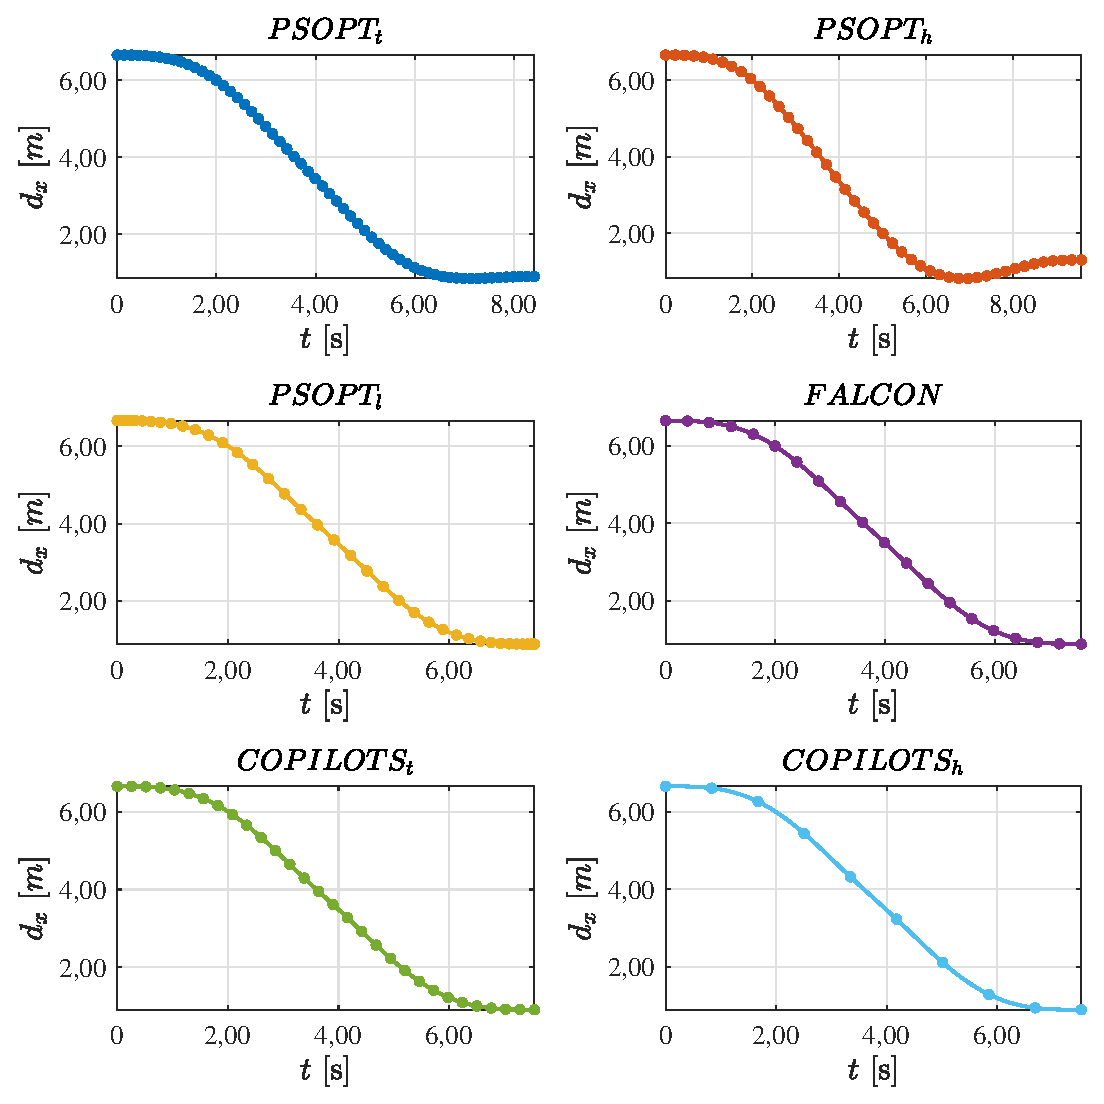
\includegraphics[scale=0.7]{fig/resultados/estacionamento/traj/x/d_x}
	\captionof{figure}[Variável de estado $d_x(t)$ para o problema do estacionamento.]{Variável de estado $d_x(t)$ para o problema do estacionamento. Os pontos representam os valores discretizados e as linhas contínuas representam as trajetórias interpoladas.}
	\label{fig:estacionamento:x:d_x}
	\vspace{\onelineskip}
\end{minipage}

\noindent
\begin{minipage}{\textwidth}
	\vspace{\onelineskip}
	\centering
	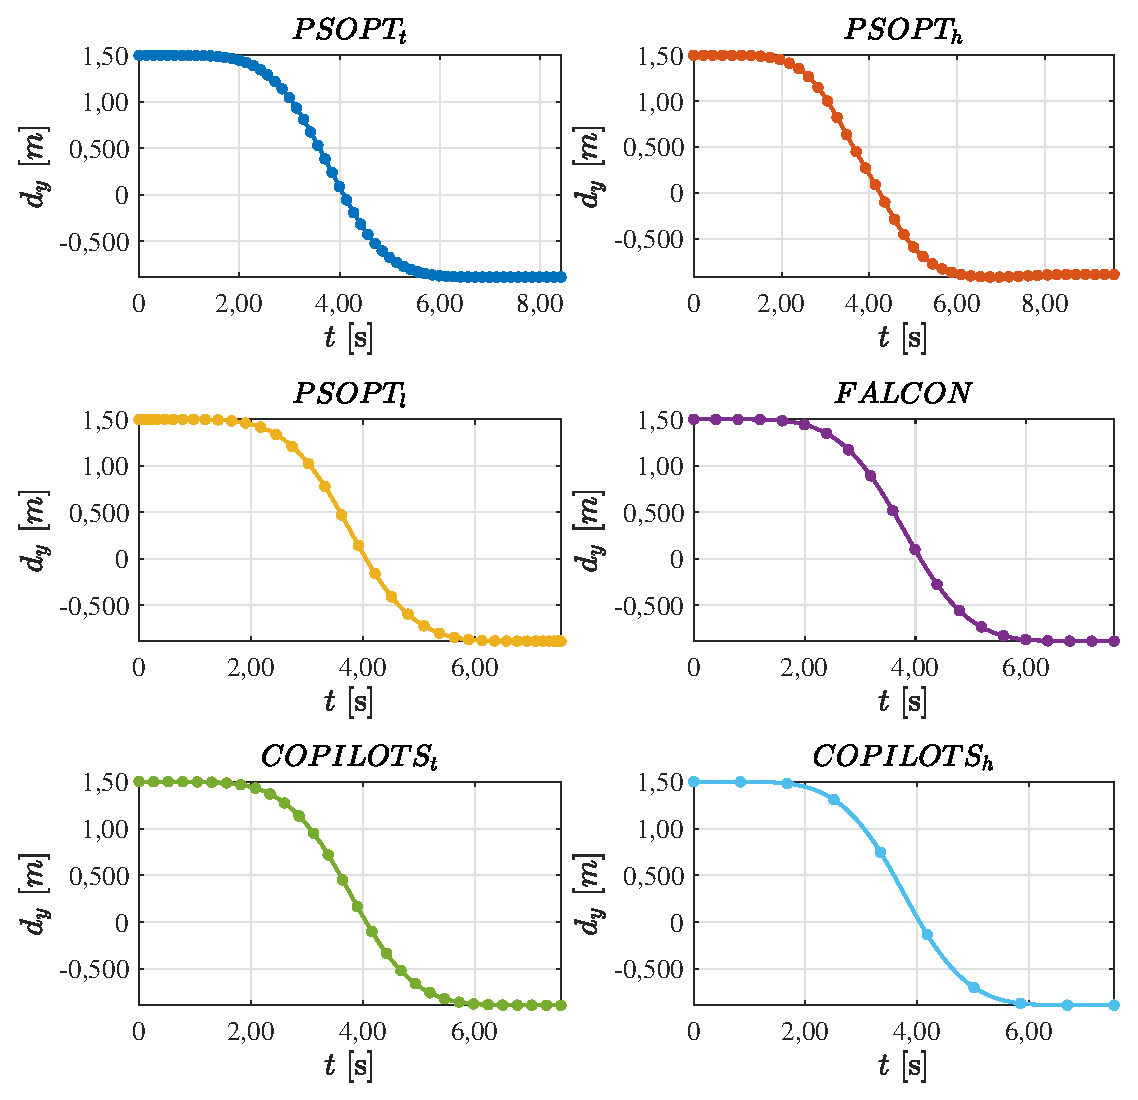
\includegraphics[scale=0.7]{fig/resultados/estacionamento/traj/x/d_y}
	\captionof{figure}[Variável de estado $d_y(t)$ para o problema do estacionamento]{Variável de estado $d_y(t)$ para o problema do estacionamento. Os pontos representam os valores discretizados e as linhas contínuas representam as trajetórias interpoladas.}
	\label{fig:estacionamento:x:d_y}
	\vspace{\onelineskip}
\end{minipage}

\noindent
\begin{minipage}{\textwidth}
	\vspace{\onelineskip}
	\centering
	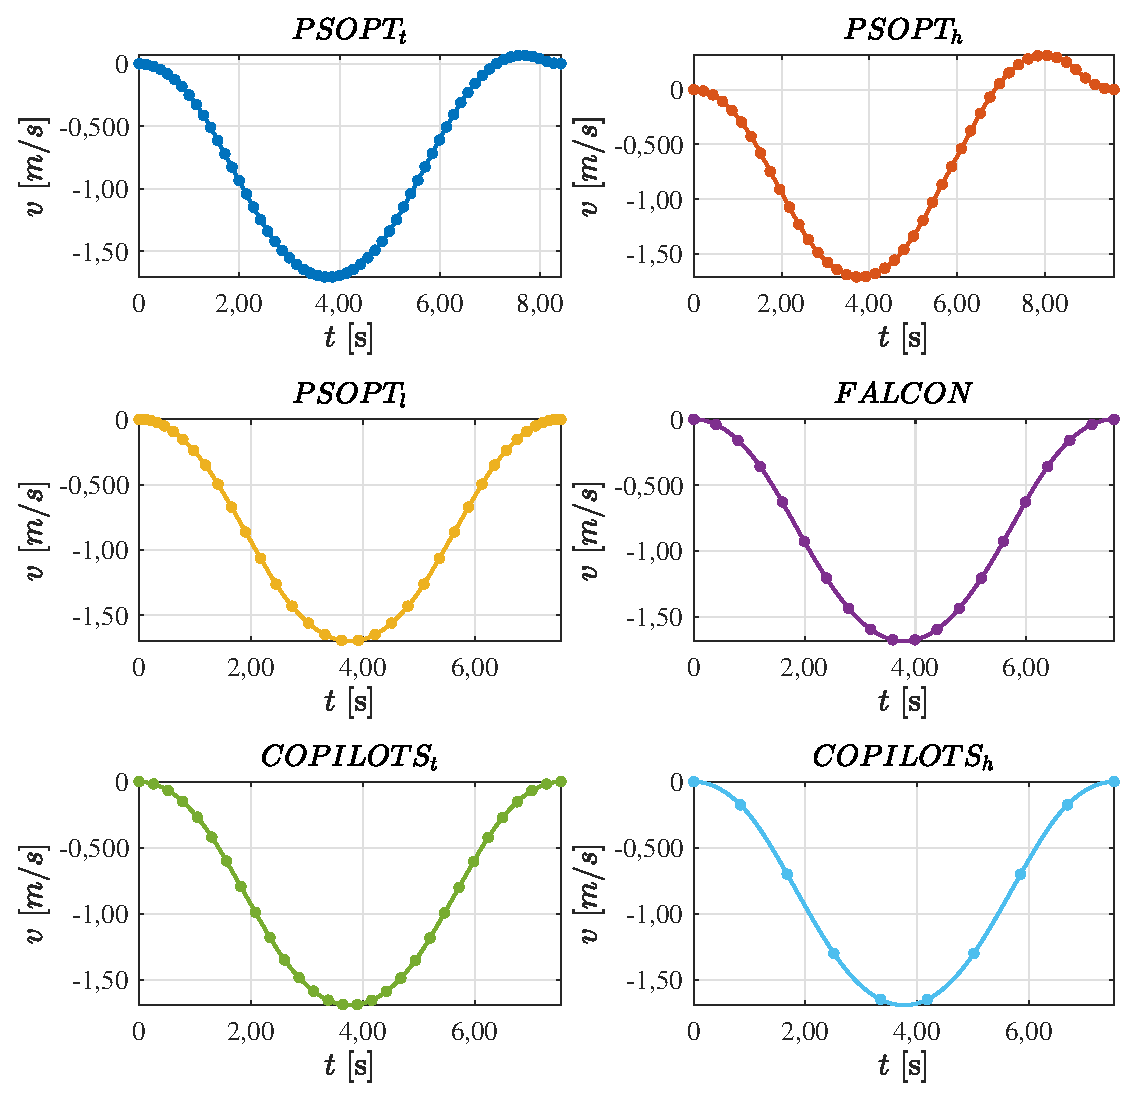
\includegraphics[scale=0.7]{fig/resultados/estacionamento/traj/x/v}
	\captionof{figure}[Variável de estado $v(t)$ para o problema do estacionamento]{Variável de estado $v(t)$ para o problema do estacionamento. Os pontos representam os valores discretizados e as linhas contínuas representam as trajetórias interpoladas.}
	\label{fig:estacionamento:x:v}
	\vspace{\onelineskip}
\end{minipage}

\noindent
\begin{minipage}{\textwidth}
	\vspace{\onelineskip}
	\centering
	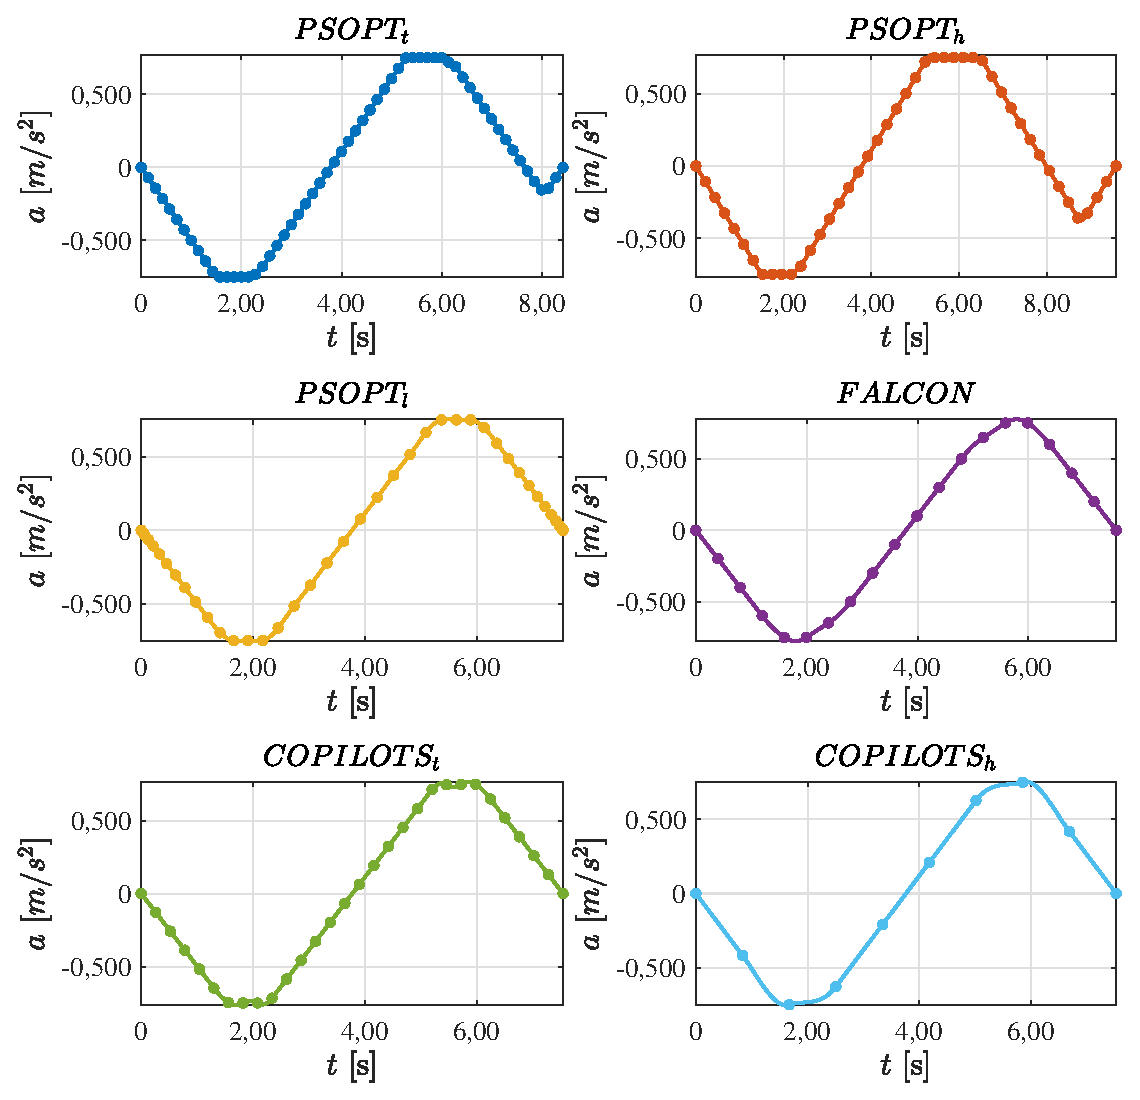
\includegraphics[scale=0.7]{fig/resultados/estacionamento/traj/x/a}
	\captionof{figure}[Variável de estado $a(t)$ para o problema do estacionamento]{Variável de estado $a(t)$ para o problema do estacionamento. Os pontos representam os valores discretizados e as linhas contínuas representam as trajetórias interpoladas.}
	\label{fig:estacionamento:x:a}
	\vspace{\onelineskip}
\end{minipage}

\noindent
\begin{minipage}{\textwidth}
	\vspace{\onelineskip}
	\centering
	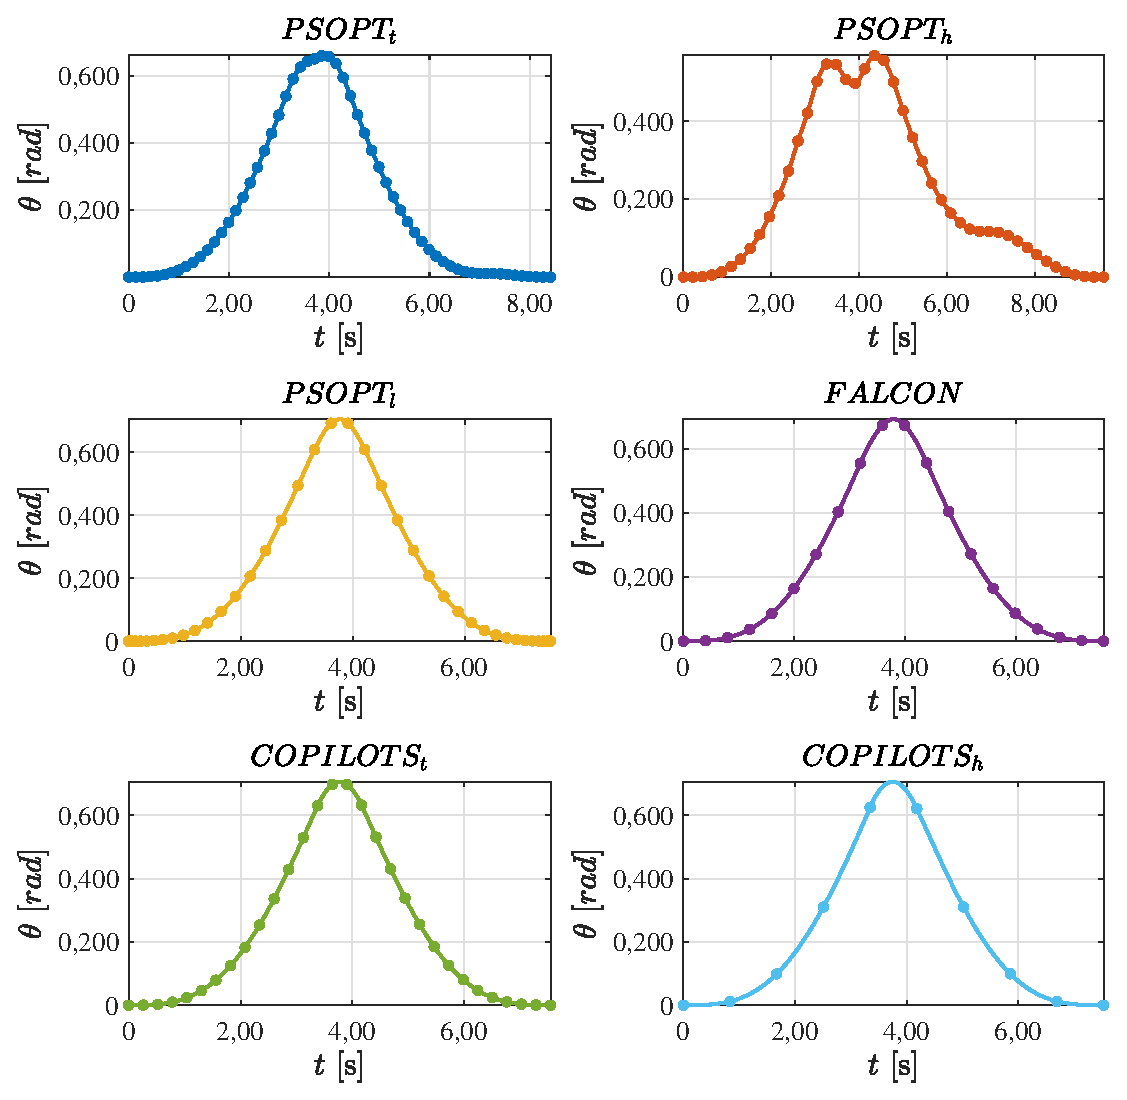
\includegraphics[scale=0.7]{fig/resultados/estacionamento/traj/x/theta}
	\captionof{figure}[Variável de estado $\theta(t)$ para o problema do estacionamento]{Variável de estado $\theta(t)$ para o problema do estacionamento. Os pontos representam os valores discretizados e as linhas contínuas representam as trajetórias interpoladas.}
	\label{fig:estacionamento:x:theta}
	\vspace{\onelineskip}
\end{minipage}

\noindent
\begin{minipage}{\textwidth}
	\vspace{\onelineskip}
	\centering
	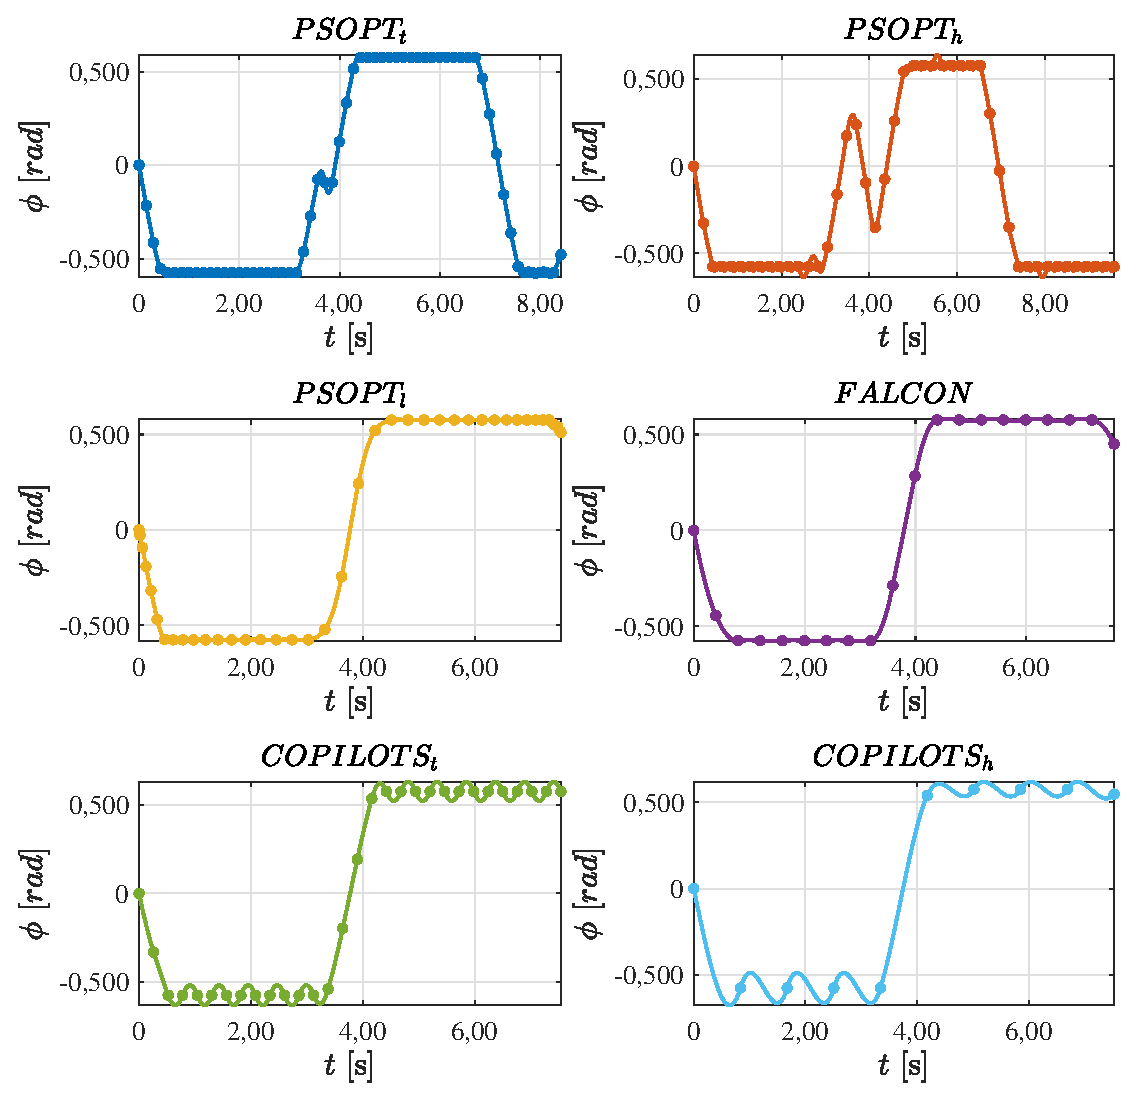
\includegraphics[scale=0.7]{fig/resultados/estacionamento/traj/x/phi}
	\captionof{figure}[Variável de estado $\phi(t)$ para o problema do estacionamento]{Variável de estado $\phi(t)$ para o problema do estacionamento. Os pontos representam os valores discretizados e as linhas contínuas representam as trajetórias interpoladas.}
	\label{fig:estacionamento:x:phi}
	\vspace{\onelineskip}
\end{minipage}

\noindent
\begin{minipage}{\textwidth}
	\vspace{\onelineskip}
	\centering
	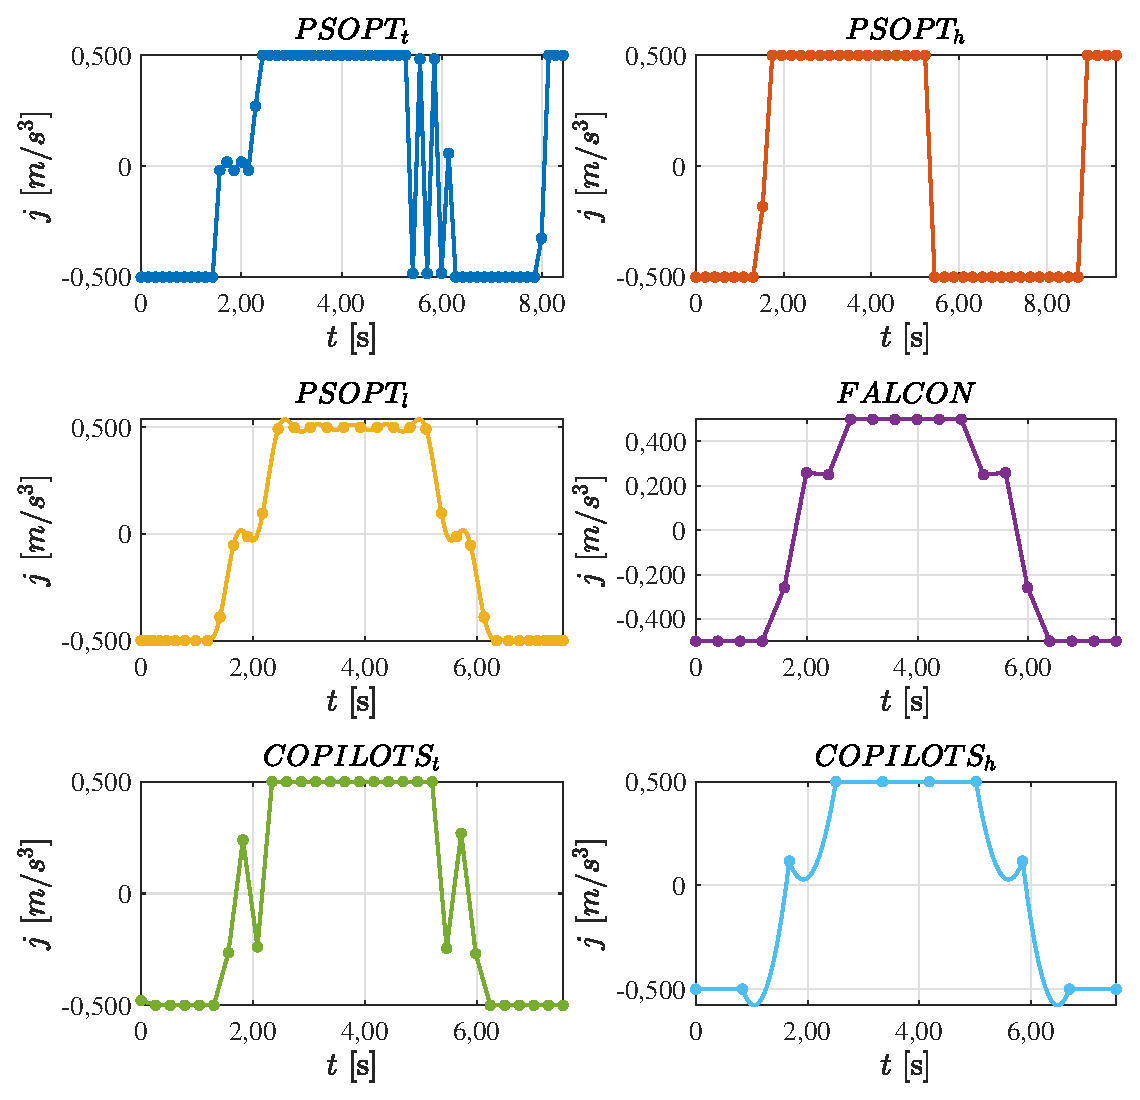
\includegraphics[scale=0.7]{fig/resultados/estacionamento/traj/u/j}
	\captionof{figure}[Variável de controle  $j(t)$ para o problema do estacionamento]{Variável de controle  $j(t)$ para o problema do estacionamento. Os pontos representam os valores discretizados e as linhas contínuas representam as trajetórias interpoladas}
	\label{fig:estacionamento:u:j}
	\vspace{\onelineskip}
\end{minipage}

\noindent
\begin{minipage}{\textwidth}
	\vspace{\onelineskip}
	\centering
	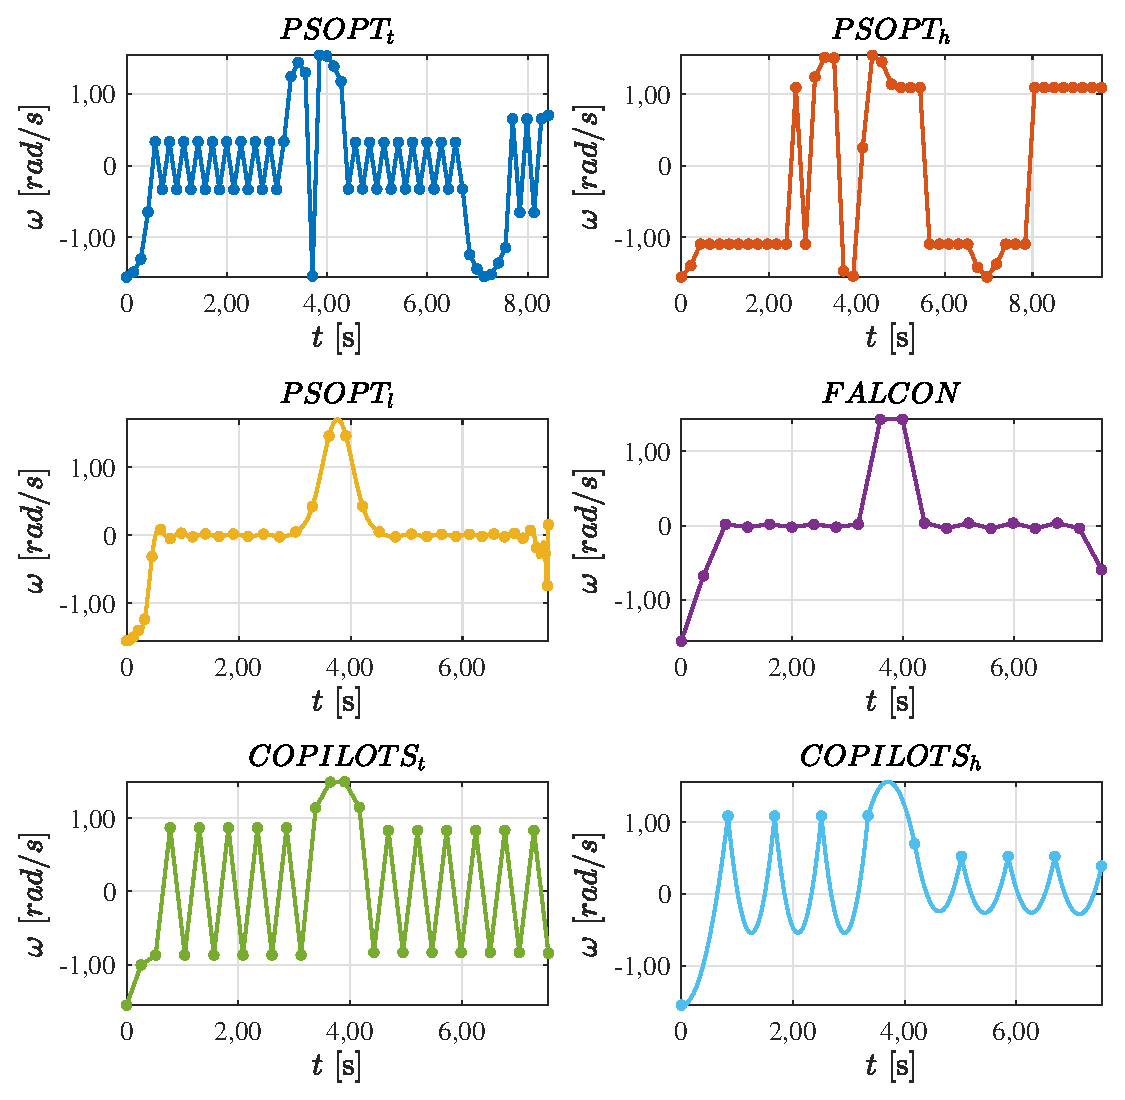
\includegraphics[scale=0.7]{fig/resultados/estacionamento/traj/u/omega}
	\captionof{figure}[Variável de controle  $\omega(t)$ para o problema do estacionamento]{Variável de controle  $\omega(t)$ para o problema do estacionamento. Os pontos representam os valores discretizados e as linhas contínuas representam as trajetórias interpoladas.}
	\label{fig:estacionamento:u:omega}
	\vspace{\onelineskip}
\end{minipage}

\todo[inline, color=pink, size=normalsize]{Análise das trajetórias de estados e controles}

Em linhas gerais, percebe-se que todos os perfis apresentam similaridades, isto é; tem a mesma tendência de comportamento. As trajetórias referentes as variáveis de estado associadas ao $PSOPT_t$ e ao $PSOPT_h$ não são perfeitamente simétricas, diferentemente das atribuídas aos demais métodos. Esse comportamento indica que mais tempo é gasto ajustando-se o veículo no interior da vaga, o que justifica os altos $t_f$ atribuídos ao $PSOPT_t$ e ao $PSOPT_h$. Já as trajetórias de $\omega(t)$ associadas a quase todos os métodos, com exceção do $PSOPT_l$ e do $FALCON$, se mostraram bastante oscilatórias, o que pode estar relacionado com às propriedades numéricas associadas às colocações trapezoidal e Hermite-Simpson. Verifica-se, inclusive uma variação bastante brusca nos $\omega(t)$ associados ao $PSOPT_t$ e ao $PSOPT_h$ em $t = 3,7$ s, o que provavelmente se deve ao uso do otimizador utilizado por este pacote. A suavidade das trajetórias encontradas pelo $PSOPT_l$ e pelo $FALCON$ se deve, provavelmente, às características numéricas inerentes à colocação pseudo-espectral e, ao emprego, por parte do $FALCON$, de ferramentas simbólicas na obtenção de derivadas analíticas. Vale ressaltar que as trajetórias de controle atribuídas a esses pacotes não apresentam oscilações de alta frequência semelhantes as verificadas nas trajetórias reportadas em \citeonline{li_time-optimal_2016}. Oscilações nas trajetórias de $\omega(t)$ levam a oscilações nas trajetórias de $\phi(t)$, uma vez que $\dot{\phi}(t) = \omega(t)$. Assim, observa-se que a amplitude das oscilações associadas à $ \phi(t) $ é particularmente alta nas trajetórias associadas ao $COPILOTS_t$ e ao $COPILOTS_h$, o que provavelmente se deve ao baixo $N_m$ atribuído a esses pacotes. No geral, as trajetórias referentes as variáveis de estado e controle obtidas pelo $PSOPT_l$ são mais suaves que aquelas determinadas pelos  demais métodos. 

Finalmente, ressalta-se que tanto os resultados aqui apresentados como aqueles reportados em \citeonline{li_time-optimal_2016} indicam a presença de variações bruscas no $j(t)$, que ocorrem em $t \approx 1,2$ s e $t \approx 6$ s. Apesar de tais variações serem inerentes à solução do estudo de caso em análise, nota-se que são especialmente acentuadas no caso do $PSOPT_h$. Além disso, verificam-se oscilações de alta frequência para $t \approx 6$ s no $j(t)$ associado ao $PSOPT_t$, o que deve estar relacionado ao otimizador, bem como às propriedades numéricas inerentes à colocação trapezoidal, uma vez que oscilações semelhantes, porém menos acentuadas, podem ser verificadas na trajetória atribuída ao $COPILOTS_t$. Vale ressaltar que a trajetória de $j(t)$ associada ao $FALCON$ é consideravelmente suave, mesmo que esse pacote empregue a colocação trapezoidal. 

\todo[inline, color=pink, size=normalsize]{Apresentação dos gráficos de trajetória complexos caso haja}

Na Figura \ref{fig:estacionamento:avancado} é apresentada a vista superior do veículo, na qual são representadas algumas das posições assumidas pelo mesmo durante a execução da manobra de estacionamento. Nesta mesma figura também é apresentada a trajetória do ponto $ P\big(d_x, d_y\big) $. A elaboração do mesmo foi baseada nos resultados obtidos pelo $ COPILOTS_h $, pacote ao qual associa-se o menor valor de $ J^* $. Nesta figura estão representadas algumas posições do veículo, bem como a trajetória ótima computada (as linhas tracejadas representam os limites da via e da vaga).  

\noindent
\begin{minipage}{\textwidth}
	\vspace{\onelineskip}
	\centering
	\includegraphics[scale=0.5]{fig/resultados/estacionamento/obs/adv}
	\captionof{figure}[Posições do veículo durante a execução da manobra no problema do estacionamento]{Posições do veículo durante a execução da manobra no problema do estacionamento.}
	\label{fig:estacionamento:avancado}
	\vspace{\onelineskip}
\end{minipage}

\todo[inline, color=pink, size=normalsize]{Apresentação das análises de sensibilidade $ N \times t_p $ e $ N \times n_{aval} $}

A influência do número de nós de colocação no tempo de processamento e no número de avaliações da função objetivo são apresentadas nas Figuras \ref{fig:estacionamento:sensibilidade:t} e \ref{fig:estacionamento:sensibilidade:naval}. Nestes gráficos são apresentadas as variações: $ \Delta t_p = \max\{t_p\} - \min\{t_p\} $ e $ \Delta n_{aval} = \max\{n_{aval}\} - \min\{n_{aval}\} $. Os pontos nos gráficos representam os valores atribuídos a $ t_p $ (e a $ n_{aval} $) para cada um dos $ N $ considerados, enquanto as linhas contínuas representam curvas de tendência, obtidas por meio de regressões lineares, em que $R^2$ é o coeficiente de determinação. Os valores de $ N $ empregados na geração desses resultados são iguais àqueles considerados na computação da relação entre $ J^* $ e $ N $. 

\noindent
\begin{minipage}{\textwidth}
	\vspace{\onelineskip}
	\centering
	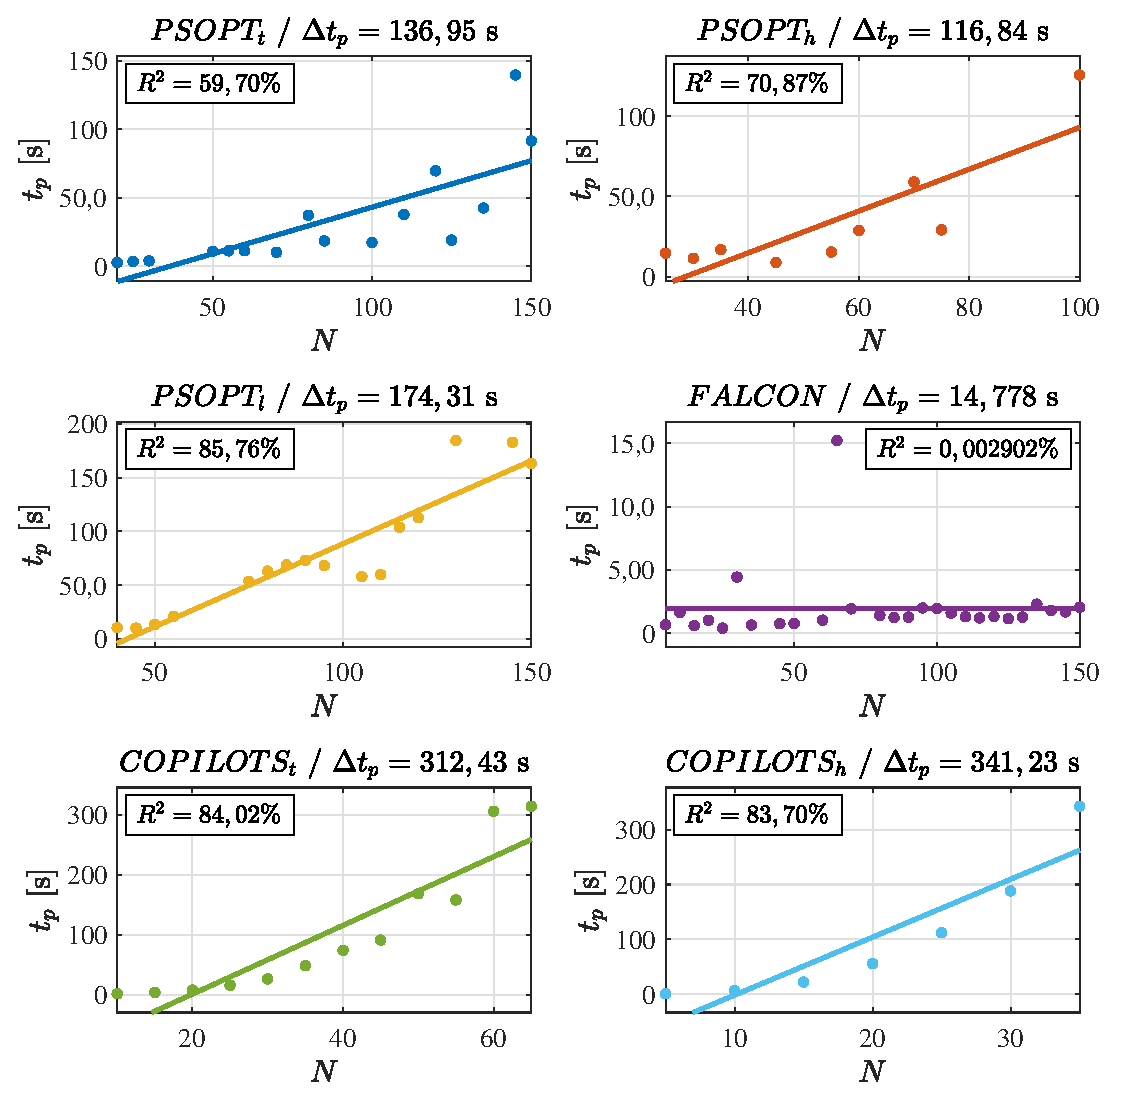
\includegraphics[scale=0.7]{fig/resultados/estacionamento/sens/t}
	\captionof{figure}[Relação entre o tempo de processamento e o número de nós de colocação no problema do estacionamento]{Relação entre o tempo de processamento $ t_p $ e o número de nós de colocação $ N $ no problema do estacionamento.}
	\label{fig:estacionamento:sensibilidade:t}
	\vspace{\onelineskip}
\end{minipage}

Primeiramente nota-se que o $t_p$ obtido pelo $FALCON$ é o menos sensível ao aumento de $N$, dado o baixo valor de $\Delta t_p$ associado a esse pacote. Em contrapartida, o $PSOPT_l$ foi o que resultou mo menor valor de $\Delta n_{aval}$. Em relação aos valores de $t_p$ e de $n_{aval}$ associados ao $FALCON$, observa-se $R^2$ especialmente baixos, uma vez que para $N = 65$, verificou-se um aumento repentino em $n_{aval}$ e, consequentemente, em $t_p$. De forma análoga, observa-se um $R^2$ consideravelmente baixo ao $n_{aval}$ associado ao $PSOPT_l$, uma vez que, nesse caso, verifica-se uma variação considerável em $ n_{aval} $ à medida que $N$ cresce, sem que seja possível verificar qualquer tendência.

\noindent
\begin{minipage}{\textwidth}
	\vspace{\onelineskip}
	\centering
	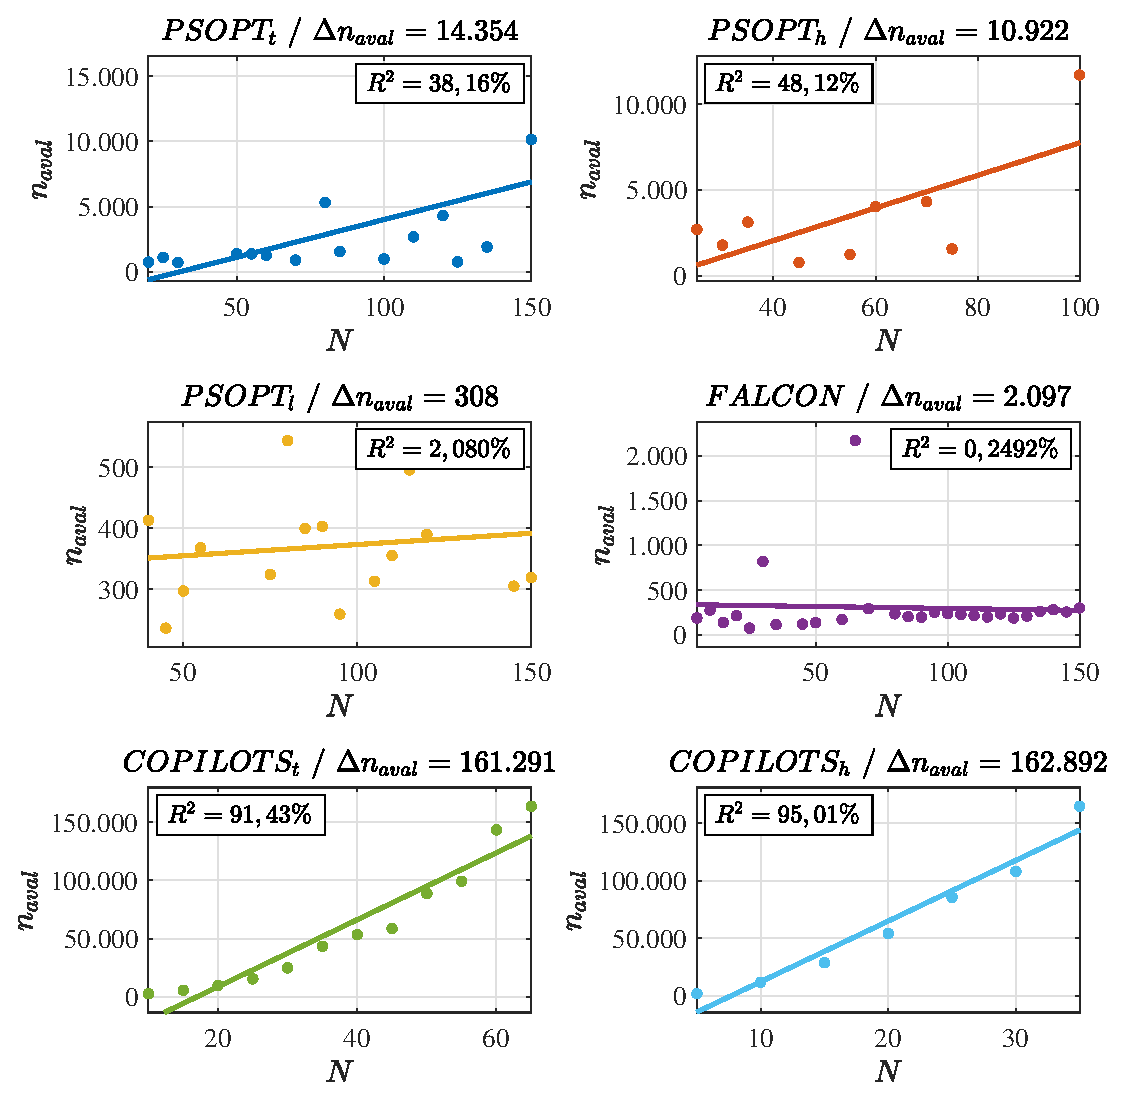
\includegraphics[scale=0.7]{fig/resultados/estacionamento/sens/eval}
	\captionof{figure}[Relação entre o número de avaliações da função objetivo e o número de nós de colocação no problema do estacionamento]{Relação entre o número de avaliações da função objetivo $ n_{aval} $ e o número de nós de colocação $ N $ no problema do estacionamento.}
	\label{fig:estacionamento:sensibilidade:naval}
	\vspace{\onelineskip}
\end{minipage}

\todo[inline, color=pink, size=normalsize]{Análise das análises de sensibilidade $ N \times t_p $ e $ N \times n_{aval} $}

Vale ressaltar que os valores de $\Delta t_p$ associados ao $PSOPT_t$, ao $PSOPT_h$ e ao $PSOPT_l$ se mostraram bastante próximos. No entanto, o mesmo não pode ser dito com relação aos valores de $\Delta n_{aval}$ associados a esses métodos. O $\Delta n_{aval}$ obtido pelo  $PSOPT_l$ é cerca de 45 vezes menor que o requerido pelo $PSOPT_t$. Ainda assim, é preciso ter cuidado ao comparar-se os resultados obtidos pelo $PSOPT_h$ e pelo $PSOPT_l$, uma vez que não foi possível, empregando-se o primeiro método, resolver o estudo de caso em análise para $N > 100$. Apesar dos altos valores de $R^2$ relacionados aos valores de $t_p$ e de $n_{aval}$ encontrados pela configurações $COPILOTS_t$ e  $COPILOTS_h$, é difícil dizer se há, nesse caso, uma relação linear entre $N$ e $t_p$ ou entre $N$ e $n_{aval}$. Tal afirmação seria equivocada considerando-se a pequena quantidade de pontos na qual foram baseadas as regressões lineares associadas a esses pacotes (12 no caso do $COPILOT_t$ e 7 no do $COPILOTS_h$). Finalmente, é preciso ter cuidado ao se comparar as sensibilidades dos parâmetros $t_p$ e $n_{aval}$ relacionados ao $COPILOTS_t$ e ao $COPILOTS_h$ com base nos valores de $\Delta t_p$ e $\Delta n_{aval}$ para cada um destes métodos, uma vez que os valores de $N_s$ encontrados são bastante distintos (iguais a 12 e 7, respectivamente). Porém, é possível dizer com segurança que os valores de $n_{aval}$ e de $t_p$ associados ao $COPILOTS$, independentemente do tipo de colocação considerada, são muito maiores que aqueles atribuídos aos demais métodos, o que se deve, provavelmente, ao uso que o pacote faz do SQP.

\todo[inline, color=pink, size=normalsize]{Observações adicionais sobre os resultados obtidos no estudo de caso}